\documentclass[12pt]{article}
\usepackage[utf8]{inputenc}
\usepackage[spanish]{babel}
\usepackage{amsmath, amssymb}
\usepackage{graphicx}
\usepackage{hyperref}
\usepackage{booktabs}
\usepackage{geometry}
\geometry{margin=2.5cm}

\title{\textbf{Simulación de Eventos Discretos\\
Modelo de Riesgo para una Compañía de Seguros}}
\author{Gabriel Alonso Coro}
\date{13 de abril de 2025}

\begin{document}

\maketitle
\tableofcontents
\newpage

\section{Introducción}

Este proyecto tiene como objetivo principal modelar y analizar el comportamiento financiero de una compañía aseguradora mediante simulación de eventos discretos. A través del desarrollo e implementación de un modelo estocástico basado en procesos de Poisson y distribuciones exponenciales, se busca evaluar el impacto de distintos parámetros clave sobre el capital final de la compañía y su riesgo de quiebra.

Se ha optado por una estrategia conservadora, priorizando configuraciones que garanticen estabilidad financiera a largo plazo con ganancias moderadas y baja probabilidad de quiebra. El enfoque experimental, apoyado en análisis de sensibilidad, permite fundamentar decisiones informadas a partir de la simulación.

\subsection*{Objetivos y metas}
\begin{itemize}
    \item Implementar un modelo de simulación de eventos discretos que represente el funcionamiento financiero de una compañía de seguros.
    \item Analizar el comportamiento del capital de la compañía en función de distintos parámetros clave.
    \item Identificar configuraciones que mantengan una ganancia moderada y minimicen la probabilidad de quiebra.
\end{itemize}

\subsection*{Variables que describen el problema}

Las principales variables involucradas en el modelo son las siguientes:

\begin{itemize}
    \item $A_0$: Capital inicial de la compañía.
    \item $c$: Prima fija que cada asegurado paga por unidad de tiempo.
    \item $\nu$: Tasa de llegada de nuevos asegurados, modelada como un proceso de Poisson.
    \item $\mu$: Tasa de salida de asegurados, inversamente proporcional al tiempo promedio que permanecen activos.
    \item $\lambda$: Tasa de generación de reclamaciones por parte de cada asegurado.
    \item $F$: Monto medio de las reclamaciones, modelado como la media de una distribución exponencial.
    \item $T$: Horizonte temporal de la simulación (días de operación del sistema).
    \item Capital final: Resultado acumulado al final del periodo simulado, en función de ingresos por primas y egresos por reclamaciones.
    \item Número de asegurados activos: Variable dinámica que cambia con las llegadas y salidas a lo largo del tiempo.
\end{itemize}


\section{Detalles de Implementación}

La simulación fue desarrollada en Python utilizando la biblioteca \texttt{SimPy}, que permite modelar sistemas de eventos discretos de manera eficiente. El proyecto está estructurado en tres directorios principales:

\begin{itemize}
    \item \textbf{src/}: Contiene el código fuente de la simulación y los análisis de sensibilidad.
    \item \textbf{data/}: Almacena los resultados de las simulaciones en archivos CSV y los gráficos generados.
    \item \textbf{docs/}: Reservado para el informe y material complementario.
\end{itemize}

La función principal de simulación recibe como parámetros la configuración del modelo (tasas de llegada, salida, reclamaciones, monto promedio, etc.) y devuelve el capital final alcanzado al concluir un horizonte de simulación de 365 días. El sistema modela la llegada de asegurados, su permanencia en la compañía, la generación de reclamaciones, y la entrada de primas, todo ello mediante distribuciones exponenciales.

Se implementó un módulo adicional que permite realizar análisis de sensibilidad sobre los parámetros principales del modelo, generando resultados estadísticos para cada configuración y gráficos comparativos.

\section{Resultados y Experimentos}

\subsection{Hallazgos de la simulación}

Tras implementar y ejecutar la simulación de la compañía aseguradora bajo diferentes configuraciones de parámetros, se obtuvieron los siguientes hallazgos principales:

\begin{itemize}
    \item \textbf{Efecto de la tasa de reclamaciones $(\lambda)$}: Valores altos de $\lambda$ incrementaron drásticamente la probabilidad de quiebra y redujeron el capital final promedio. En cambio, valores muy bajos dieron lugar a ganancias excesivas, ajenas a la estrategia conservadora. Un equilibrio se encontró alrededor de $\lambda = 0.095$.
    \item \textbf{Efecto de la tasa de llegada $(\nu)$}: Se observó que a mayor $\nu$, mayor era el capital promedio, pero también la variabilidad y, en ciertos casos, la probabilidad de quiebra. La tasa de llegada $\nu = 3$ resultó apropiada para mantener ganancias moderadas con bajo riesgo.
    \item \textbf{Efecto de la tasa de salida $(\mu)$}: Tasas de salida más altas $(\mu > 0.3)$ propiciaron ganancias más moderadas y menor probabilidad de quiebra, al equilibrar la permanencia de los asegurados y el ingreso de primas.
    \item \textbf{Efecto del monto medio de reclamación $(F)$}: Valores superiores a 100\$ incrementaron el riesgo de quiebra. En cambio, un valor cercano a 100\$ mantuvo el capital dentro del rango deseado de \$500--\$3000 y con una quiebra menor al 10\%.
\end{itemize}

A partir de estas observaciones, se definió como configuración final:
\[
A_0 = 1000,\quad c = 10,\quad \nu = 3,\quad \mu = 0.4,\quad 
\lambda = 0.095,\quad F = 100,\quad T = 365.
\]

En promedio, esta configuración produjo un capital final de \$2624 con un 6.7\% de probabilidad de quiebra, cumpliendo con el enfoque prudente de mantener ganancias moderadas y bajo riesgo.

\subsection{Interpretación de los resultados}

El comportamiento del sistema bajo diferentes parámetros confirma la importancia de mantener un balance entre las tasas de entrada y salida de asegurados, así como en la generación y el monto de las reclamaciones. Desde la postura conservadora adoptada, las simulaciones indican que:

\begin{itemize}
    \item Una \emph{tasa de reclamaciones} moderada $(\lambda \approx 0.095)$ evita tanto la quiebra masiva como ganancias excesivas.
    \item Una \emph{tasa de llegada} controlada $(\nu = 3)$ previene aumentos desproporcionados del capital y, por ende, se alinea con la idea de ganancias moderadas.
    \item Una \emph{tasa de salida} relativamente alta $(\mu = 0.4)$ reduce la permanencia de los asegurados, lo que estabiliza el capital y disminuye la dispersión de los resultados.
    \item Un \emph{monto medio de reclamación} de \$100 se adecua al criterio de bajo riesgo, ya que valores mucho mayores disparan la probabilidad de quiebra.
\end{itemize}

Estos resultados permiten inferir que la compañía se mantendría financieramente estable en un horizonte anual, sin aspirar a ganancias máximas pero con una probabilidad de quiebra razonablemente baja.

\subsection{Hipótesis extraída de los resultados}

A partir de los hallazgos anteriores, se puede enunciar la siguiente hipótesis:

\begin{quote}
\emph{``Bajo un enfoque conservador, existe un rango moderado de valores para $\lambda$, $\nu$, $\mu$ y $F$ que mantiene el capital final de la compañía de seguros en un nivel estable (entre \$500 y \$3000) y minimiza el riesgo de quiebra (por debajo del 20\%).''}
\end{quote}

Se espera que, al apartarse de este rango, el sistema ya sea sufra quiebras con mayor frecuencia o presente ganancias excesivamente altas, rompiendo la estrategia prudente planteada.

\subsection{Experimentos realizados para validar la hipótesis}

Para validar la hipótesis, se llevaron a cabo \textbf{experimentos de sensibilidad} en los que se variaron uno a uno los principales parámetros:

\begin{itemize}
    \item \textbf{Tasa de reclamaciones $(\lambda)$}: Se probó entre 0.09 y 0.11.
    \item \textbf{Tasa de llegada $(\nu)$}: Valores desde 3 hasta 9.
    \item \textbf{Tasa de salida $(\mu)$}: Valores de 0.1 a 0.4.
    \item \textbf{Monto medio reclamado $(F)$}: De \$90 a \$110.
\end{itemize}

En cada configuración se corrieron 30 réplicas de la simulación, registrando el capital final, su desviación estándar y la proporción de réplicas con capital negativo. Al analizar los resultados, se comprobó que la hipótesis se sostiene: valores extremos en los parámetros conllevan ya sea quiebras frecuentes o ganancias excesivas.

\begin{figure}[h!]
    \centering
    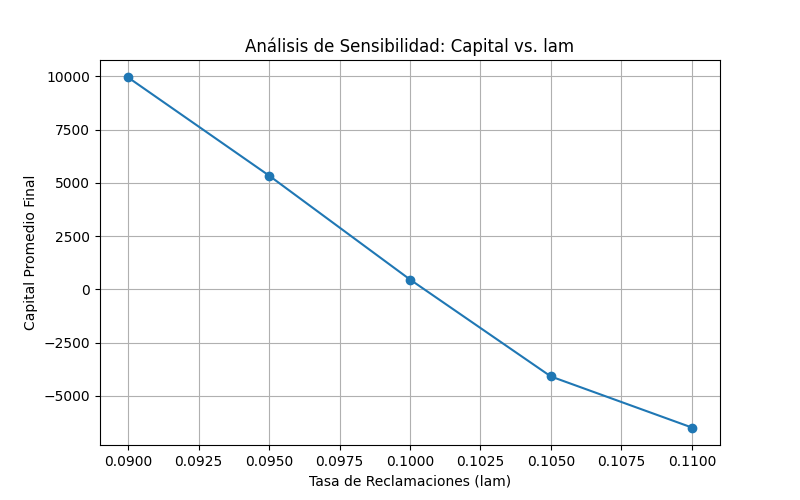
\includegraphics[width=1.1\textwidth]{sensibilidad_lam.png}
    \caption{Capital promedio en función de la tasa de reclamaciones $\lambda$.}
    \label{fig:sensibilidad_lam}
\end{figure}

\begin{figure}[h!]
    \centering
    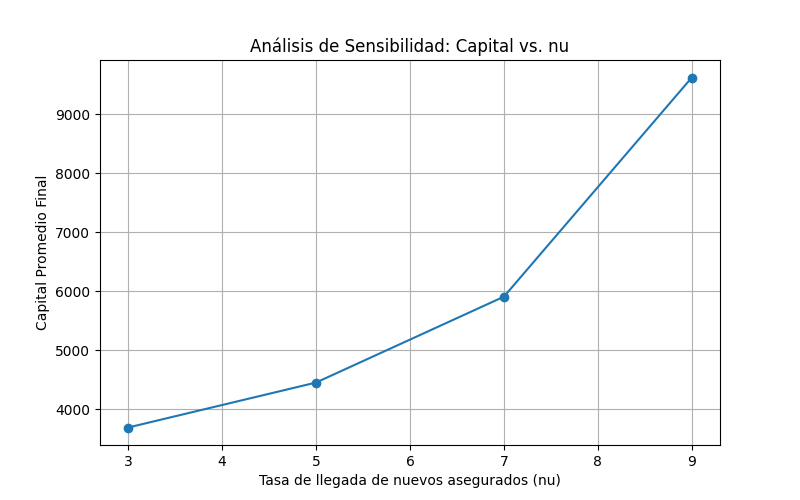
\includegraphics[width=0.9\textwidth]{sensibilidad_nu.png}
    \caption{Capital promedio en función de la tasa de llegada de asegurados $\nu$.}
    \label{fig:sensibilidad_nu}
\end{figure}

\begin{figure}[h!]
    \centering
    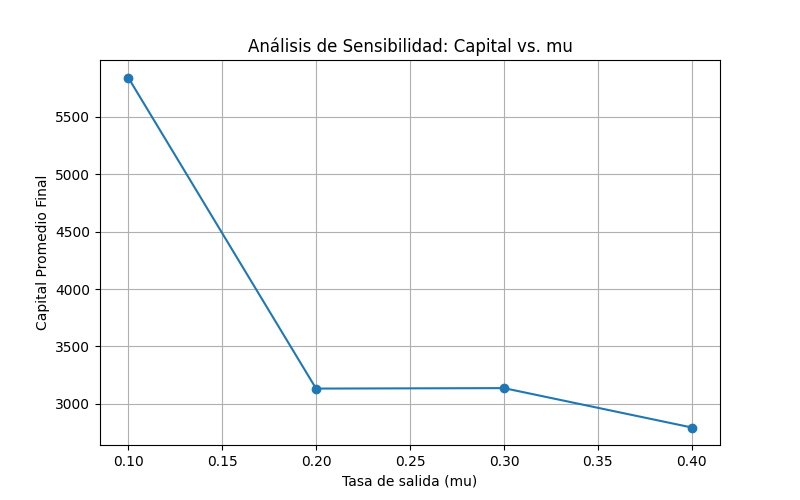
\includegraphics[width=0.9\textwidth]{sensibilidad_mu.png}
    \caption{Capital promedio en función de la tasa de salida de asegurados $\mu$.}
    \label{fig:sensibilidad_mu}
\end{figure}

\begin{figure}[h!]
    \centering
    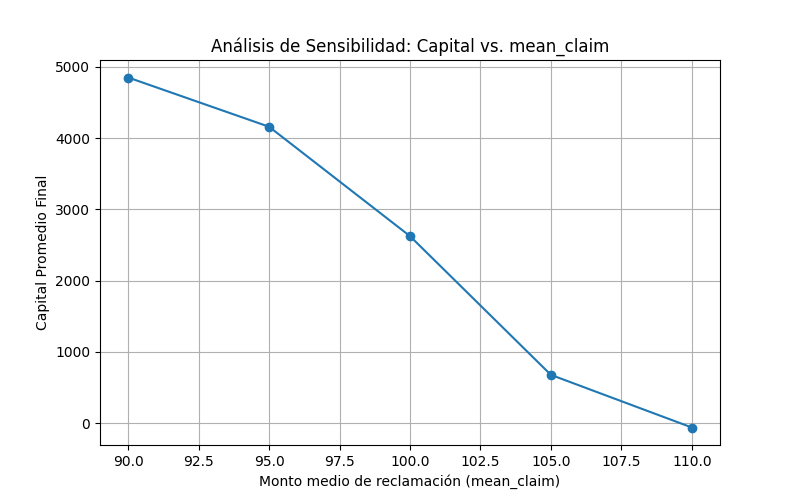
\includegraphics[width=0.9\textwidth]{sensibilidad_mean_claim.png}
    \caption{Capital promedio en función del monto medio de las reclamaciones $F$.}
    \label{fig:sensibilidad_mean_claim}
\end{figure}

\subsection{Necesidad de realizar el análisis estadístico de la simulación (variables de interés)}

Dado el carácter estocástico de la simulación, cada conjunto de valores de parámetros produce diferentes resultados en distintas réplicas. Por ello, resultó fundamental calcular:

\begin{itemize}
    \item \textbf{Media del capital final}: refleja la tendencia central de las ganancias.
    \item \textbf{Desviación estándar}: cuantifica la dispersión y el riesgo potencial.
    \item \textbf{Porcentaje de quiebra}: la fracción de réplicas que cerraron con capital negativo.
\end{itemize}

Estas métricas permiten una visión integral del desempeño, evitando conclusiones basadas únicamente en la media del capital. La variabilidad y el porcentaje de quiebra arrojan luz sobre la estabilidad real del sistema.

\subsection{Análisis de parada de la simulación}

Para simplificar, se estableció un horizonte fijo de 365 días de operación. \emph{No se implementó} una condición de parada anticipada en caso de quiebra o saturación de recursos. Sin embargo, en estudios futuros podría considerarse detener la simulación en el momento exacto en que el capital se vuelve negativo, o cuando los ingresos y egresos se estabilizan, si el objetivo es examinar el comportamiento a más largo plazo.



\section{Modelo Matemático}

\subsection*{Supuestos del modelo}
\begin{itemize}
    \item Los asegurados llegan según un proceso de Poisson con tasa $\nu$.
    \item Cada asegurado permanece en la compañía por un tiempo exponencial con tasa $\mu$.
    \item Mientras permanece activo, cada asegurado realiza reclamaciones según un proceso de Poisson con tasa $\lambda$.
    \item Los montos de las reclamaciones siguen una distribución exponencial con media $F$.
    \item Cada asegurado paga una prima fija $c$ por unidad de tiempo.
    \item El capital de la compañía se actualiza en función del ingreso por primas y el egreso por reclamaciones.
\end{itemize}

\subsection*{Restricciones}

No se modelaron costos fijos, beneficios adicionales ni interacción entre asegurados. La simulación no contempla escenarios con interrupciones externas ni eventos catastróficos. Se asume independencia entre asegurados.

\subsection*{Comparación entre resultados esperados y simulados}

Dado que no se cuenta con datos reales para contrastar, se realizaron comparaciones internas entre configuraciones simuladas para evaluar su estabilidad y razonabilidad. El comportamiento observado es consistente con la teoría: a mayores tasas de reclamación y mayores montos medios, se reduce el capital promedio y aumenta la probabilidad de quiebra.

\section{Conclusiones}

La simulación implementada permite comprender cómo afectan los parámetros clave al comportamiento financiero de una compañía de seguros. La estrategia conservadora adoptada resultó efectiva para identificar configuraciones que aseguran estabilidad económica con un riesgo de quiebra aceptable.

Mediante análisis de sensibilidad se concluyó que tasas de llegada bajas, junto a tasas de reclamaciones moderadas y montos medios controlados, son esenciales para evitar escenarios de pérdida.


\end{document}
